\subsubsection{Projekt verwalten}
\begin{figure}[H]
  \begin{center}
    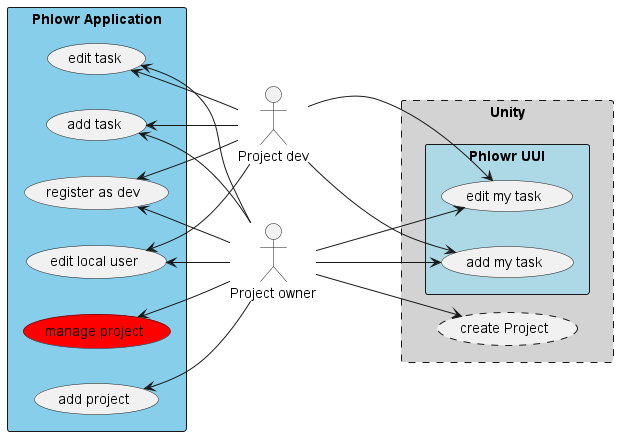
\includegraphics[width=0.3\linewidth]{../content/diagrams/usecase/overview/overviewUseCaseManageProjectSelected.png}
    \caption{Use Case Diagaramm <manage project> }
  \end{center}
\end{figure}

\begin{table}[H]
    \centering
    \settowidth\tymin{executeIncomingCommand()}
    \setlength\extrarowheight{2pt}
    \begin{tabulary}{1.0\textwidth}{|m{4cm}|m{9cm}|}
      \hline
      \textbf{Use Case} &
      \textbf{MANAGE PROJECT}\\
      \hline
      \textbf{Beschreibung} &
      Ein Projekt wird in der applikation verwaltet\\ 
      \hline
      \textbf{Includes} &
      \begin{itemize}
        \item Beschreibung anpassen (edit description)
        \item Name anpassen (edit name)
        \item User-Slots anpassen (edit user-slots)
        \item Projekt-Owner ändern (change PO)
        \end{itemize}\\ 
      \hline 
      \textbf{Akteure} &
      Projekt-Owner\\ 
      \hline
      \textbf{Auslöser} &
      Ein Projekt soll angepasst werden\\ 
      \hline
      \textbf{Vorbedingungen} &
      Das Projekt wurde der Applikation hinzugefügt und der ausführende User ist der Project-Owner\\ 
      \hline
      \textbf{Abschlussbedingungen} &
      Die gewünschten Änderungen wurden gemacht und das Projekt wurde gespeichert\\ 
      \hline
      \textbf{Ablauf} &
      \begin{enumerate}
        \item Applikation öffnen
        \item <Projekt Editieren> wählen
        \item Gewünschte Änderungen vornehmen (siehe Includes)
        \item Speichern
        \end{enumerate}\\ 
      \hline
      \textbf{Zu Beachten / Notizen} &
      \begin{itemize}
        \item Projekte dürfen nur vom PO editiert werden können
        \end{itemize}\\ 
      \hline
    \end{tabulary}
    \caption{Use Case: MANAGE PROJECT}
  \end{table}